\documentclass[11pt]{report}
\usepackage{graphics}
\usepackage{graphicx}
\usepackage{epsfig}
\usepackage{fancyhdr}
\usepackage{fullpage}
\usepackage{titlesec}% http://ctan.org/pkg/titlesec
\setcounter{secnumdepth}{3}

\begin{document}
\renewcommand\bibname{References}
\pagestyle{fancy}
\fancyhead{}
\fancyfoot{}
\fancyfoot[c]{\thepage}
\fancyfoot[l]{B.Tech CS 2013-17}
\lhead{abcd}
\renewcommand{\chaptermark}[1]{
\markboth{\thechapter.\ #1}{}} 
\renewcommand{\headrulewidth}{0.3pt}
\fancyhead[r]{\slshape \leftmark}
\addtolength{\headheight}{\baselineskip}

\lhead{\nouppercase{\rightmark}}
\rhead{\nouppercase{\leftmark}}
\lhead{RentaHoliX} % <====short project title here
%\fancyhead[LO,RE]{\slshape \leftmark}
%\bibliographystyle{plain}
\title {RentaHoliX}
\author{Group No. 10\\\\12140825 HARIKISHEN H\\ 12140819 DEON SUNNY\\ 12140816 ATHUL RAJ T S\\ 12140837 NARENDRAN T\\...\\}
%\maketitle

\begin{titlepage}
\begin{center}

%\topmargin100pt
\Huge{\textbf{RentaHoliX}}\\
\vspace{0.05in}
\large{\textbf{CS 16L2 Mini Project\\}}
\vspace{1.2in}



\begin{center}

\Large{\textbf{12140816}}  \Large{\textbf{ATHUL RAJ T S}}\\ 
\Large{\textbf{12140820}}  \Large{\textbf{DEON SUNNY}}\\ 
\Large{\textbf{12140825}}  \Large{\textbf{HARIKISHEN H}}\\
\Large{\textbf{12140840}}  \Large{\textbf{NARENDRAN T}}\\

\end{center}

\Large{\textbf{
B.Tech Computer Science \& Engineering
}}


\vspace{2.0in}
\begin{figure}[h]
\begin{center}
%\epsfig{width=1in, file=embN1.jpg}

\epsfig{width=1.25in, file=logo.jpg}

\end{center}
\end{figure}
%\vspace{.2in}
\textbf{
Department of Computer Engineering\\
Model Engineering College, Thrikkakara\\
Kochi 682021\\
Phone: +91.484.2575370\\
http://www.mec.ac.in\\
hodcs@mec.ac.in\\
\vspace{0in}
{\footnotesize APRIL 2016}
}
\end{center}
\end{titlepage}



%=================================================================================

\begin{titlepage}
\begin{center}
\Large{\textbf{Model Engineering College, Thrikkakara}}\\
\Large{\textbf{Dept. of Computer Engineering}}\\
\end{center}
\begin{figure}[h]
\begin{center}

\epsfig{width=1.75in, file=logo.jpg}
\end{center}
\end{figure}
\begin{center}
\Large{\textbf{C E R T I F I C A T E}}\\
\vspace{.1in}
\end{center}
This is to certify that, this report titled \textbf{\textit{RentaHoliX}} is a bonafide record of the work done by\\
\begin{center}

\Large{\textbf{12140816}}  \Large{\textbf{ATHUL RAJ T S}}\\ 
\Large{\textbf{12140820}}  \Large{\textbf{DEON SUNNY}}\\ 
\Large{\textbf{12140825}}  \Large{\textbf{HARIKISHEN H}}\\
\Large{\textbf{12140840}}  \Large{\textbf{NARENDRAN T}}\\

\end{center}
\centerline {\textsf{Sixth Semester B. Tech Computer Science \& Engineering}} students, for the course work in \textbf{CS 16L2 Mini Project},  under our guidance and supervision, in partial 
fulfilment of the requirements for the award of the degree, B. Tech Computer Science  and Engineering of \textbf{Cochin University of Science \& Technology}.
\vspace{.1in}
\begin{tabbing}
xxxxxxxxxxxxxxxxxxxxxxxxxxxxxxxxxxxxxx\= xxxxxxxxxxxxxxxxxx\= \kill

Guide			\>				\> Coordinator \\
\end{tabbing}
\begin{tabbing}
xxxxxxxxxxxxxxxxxxxxxxxxxxxxxxxxxxxxxx\= xxxxxxxxxxxxxxxxxx\= \kill
\vspace{.1in}\\		
Vineetha K.V \> \> Jaimon Jacob \\
Asst. Professor	\> \> Asst. Professor\\
Computer  Engineering	\>	\> Computer  Engineering\\
\end{tabbing}
\vspace{.1in}
%
\begin{tabbing}
xxxxxxxxxxxxxxxxxxxxxxx\= xxxxxxxxxxxxxxxxxx\= \kill

			\>Head of the Department \\

\\ 22-04-2016
%\begin{center}
\> Manilal D L\\
\> Associate Professor\\
\> Computer  Engineering\\
%\end{center}
\end{tabbing}
\end{titlepage}
  
%========================================================================================
 

\begin{titlepage}
%\pagebreak
\vspace{.25in}	
\begin{center}
\Large\textbf{{Acknowledgments}}\\
\end{center}
%\LARGE{Acknowledgment}\\
\normalsize
\vspace{.25in}

\vspace{.25in}
At this moment of accomplishment, as we are presenting our work with great pride and pleasure,
we would like to express our sincere gratitude to all those who helped us in the successful completion
of this venture. First of all, we would like to thank our Principal \textbf{Prof. Dr. V.P. Devassia} for
providing us with a conductive environment and requisite lab facilities. We wish to express our
sincere thanks to \textbf{Mr. Manilal D L} , Head of the Department, Computer Science and
Engineering, for his inspiration and constant encouragement which made us take up the project
and bring it to the completion. We are indebted to our project coordinator \textbf{Mr. Jaimon Jacob},
Assistant Professor, Department of Computer Science and Engineering, for his constant help and
support. We extend our sincere and heartfelt thanks to our guide \textbf{Mrs. Vineetha K V} for helping
us throughout the course of this project by providing us with valuable advice and suggestions.
We also take this opportunity to specially thank our Parents and Friends for their motivation,
encouragement and for being a constant support throughout. Above all we thank God Almighty
for giving us the courage to move forward with confidence and for all his blessings throughout.

\begin{flushleft}
\small{\texttt{Athul Raj T S}}\\
\small{\texttt{Deon Sunny}}\\
\small{\texttt{Harikishen H}}\\
\small{\texttt{Narendran T}}
\end{flushleft}
 
\end{titlepage}

%=================================================================== 
 
\begin{abstract}
\pagenumbering{roman}

This mini project aims at creating an e-Commerce portal for renting out products. Both people who intend to rent out their less used products for a few days, months, or years and those who intend to rent them can register in this website. The website provides facility to post details of products such as cameras, bikes, cycles, lawn mowers etc that are to be rented out. The buyers and renters are matched mainly based on location, period of rental, and expected rent amount. This website can be extremely useful in scenarios such as the following :-
Suppose you are planning on a long business trip and have a bike which could be rented out , thereby being an extra source of income and the bike won't be damaged due to not using it for a long time.
\end{abstract}

\tableofcontents

%===============================================================

\chapter {Introduction}
\label{intro}

\pagenumbering{arabic}
 
\textbf{RentaHoliX} - This Online Product Rental Portal is a web based application for people to rent-out and rent-in products at the leisure of their homes. It provides a User-Friendly interface which can be accesed using a web browser. People can rent-out their stuff by providing details of the product such as sample images, expected rent, name, description etc. Users can rent-in products by logging in to the web app providing necessary details and by paying a initial deposit amount. Users need not register to browse through the various products available for renting, but for rent-out and rent-in sign-up/registration is necessary. Products can be searched for category-wise and also, results can be filtered based on location, rent, bonds etc.\\   


Renting is a sensible way to enjoy life, while reducing our impact on the planet, our home. Every time you rent something it’s a product which doesn’t get made, packaged, shipped and sold.

%optional 
 
 
%=================================================================

\chapter {Literature Survey}
\label{ls}
 
\section{ Existing Systems}
In the existing systems, people have to buy products they want and sell them if they don't use them anymore. The issues regarding this is that even if someone wants a particular product for small periods of time they have to buy them. This may not be a problem for small things but can be expensive for larger products. In the case of selling, there is a large possibility of loss.
\subsection{Limitations of Existing Systems}
\begin{itemize}
  \item Buying products is not a viable solution for temporary use.
  \item Selling products may lead to unprecedented loss.
  \item Buying/Selling is a one off process.
  \item A product which may be useful later but not now cannot be sold.
\end{itemize}


\section{Proposed System}
 The proposed system is an online product rental portal with which a user can create an account, using which he/she can rent-out and rent-in products on per day/per week/per month basis. If he/she wants to rent out a product, he/she must provide the basic details of the product alongwith images, description, cost and the intended rent. If he/she wants to rent-in a product, he/she must place a rent request upon which an E-mail will sent to both renter/rentee. He/She can verify the product physically, place the deposit amount and approve it in the web app. He/She can only rent an available product. When the product is returned, the renter has to approve inorder refund the deposit amount. Also the renter can request a return for a rented product. Login is not necessary to browse/search products. Also, automated mails are sent for various actions such as on signup, rent-in, rent-out, posting complaints, adding products etc.
\subsection{Advantages of Proposed System}
\begin{itemize}
  \item Renting is a good solution for short as well as long periods as the product can be returned and/or can be requested back if a need for it arises later on.
  \item Renting a product makes it a form of passive revenue.
  \item Renting products can be helpful for people relocating for a short span.
  \item Product will generally be in good shape as it doesn't stay unused for a prolonged interval. 
  \item Unnecessary wastage of space with unusable products will be reduced.
\end{itemize}
 
%======================================================= 
 
\chapter {Proposed System}
\label{ps}

\section{Problem Statement}

To create an E-Commerce portal to facilitate renting out less used or spare products to willing people. It matches based on location, expected rent etc.

\section{Proposed Solution}

The proposed online portal consists of the following options :-
\subsection{Admin and User Authentication}
A privileged user can access the admin page with his/her username and password. This user has access to all user, product, and transaction details.
\\Other users must register/sign-up and login inorder to rent-out/rent-in products. But users must be able to browse products without log-in.
\subsection{Posting Details}
A user who wants to rent out a product must first register/login to the web app. The registered users must have an option to edit their personal details.
The facility to post details of a product including short description, expected rent, images etc. Moreover, the renters must have an option to edit/remove the details of products they have rented out. Also, a post may be automatically removed on expiry of rental period specified by the renter.
\subsection{Categorized Navigation }
Grouping of products based on category and an interface to navigate between them.

\subsection{Renting Products}
When a user wants to rent a product, he/she can search for the product in the relevant sections. On finding the required product, a list of all available offers will be shown which can be further filtered based on location, rating, expected rent etc. The user can then select a suitable offer.
He/she must then proceed to put a request alongwith paying a deposit amount. On acceptance by the renter, the rentee will be contacted by the agency.
\subsection{Automated Mail}
An e-mail will be automatically generated and sent to the renter when a request for his/her product is received. A mail will also be sent to the rentee  when the request has been accepted. A mail will also be generated to either the renter or the rentee when a complaint regarding a transaction has been submitted. 
\subsection{\label{mlr}Report Issues}
A rentee can report issues regarding a renter or the web app. The renter/rentee can report bugs or issues with the web app. \\

\subsection{\textbf{Input:}}
\begin{itemize}
  \item User credentials for registration/login to the web app.
  \item Product details with images.
  \item Payment Details for deposit payment.
  \item Reviews/Complaints of products.
  \item Product Rating.
  \item Search string.
\end{itemize}


\subsection{\textbf{Output:}} %expected output/outcome
\begin{itemize}
  \item User account details.
  \item Product details.
  \item Search results.
  \item Reviews of products.
  \item Product Rating.
  \item Transaction response.
  \item About Us.
  \item Help and Rules of Usage.
\end{itemize}

%======================================================= 
 
\chapter {Software Requirement Specification}
\label{srs}

% refer your SRS report

\section{Introduction}
\subsection{Purpose}
The purpose of this document is to provide a detailed description of the Online Product Rental Portal. It 
explains the purpose and features of the application, it's interfaces, functions, the constraints under which it 
must operate and how the system will respond to external stimuli. This document is intended for both the 
users and the developers of the system.
\subsection{Intended audience}
This document is intended equally for both the developers, the users of the application, the staff and 
students.
\subsection{Project Scope}
This software provides an online interface for users to rent­in and rent­out products. Users can rent­in 
products for short­term usage rather than buying them. It can also be a means of passive income for the 
renters. Furthermore, a location based search module is provided in order to facilitate product rental in a 
specific location.
\section{Overall Description}
\subsection{Product Perspective}
The software is a new self­contained product. It consists of three parts – a web interface, a back­end script 
and a database. 

\subsection{Product Functions}
This software's main functions include providing an easy to use interface for users, transaction management, 
product rental, product addition, automated mail, user and admin authentication and a search function.
\subsection{Operating Environment}
The application is designed to run on all existing mainstream web browsers such as (Google Chrome, 
Mozilla Firefox etc).
\subsection{Design and Implementation Constraints}
\begin{itemize}
  \item Expansion of the software onto a larger user base may lead to server failure.
  \item Uploading large size images may cause memory shortage.
  \item As the application involves payment and billing, certain security issues can arise.
\end{itemize}

\subsection{Assumptions and Dependencies}
It is assumed that the number of active users at any time will be less than the maximum number the server 
can handle. Also, it is assumed that one of the browsers specified in the operating environment section of 
this document will be used.
\section{External Interface Requirements}
\subsection{Software Interfaces}
A back end script is required to interface the web front end and the database. Also a script to interface the 
application and the payment gateway is required.
\subsection{Communication Interfaces}
The response of the computations done with the user input is an HTML  page. Asynchronous data transfer 
from the front­end and back­end is done using JSON format. The following protocols are used: HTTP, 
HTTPS. Also, the SMTP is used for automated e­mails.
%%%%%
\section{Functional Requirements}

\subsection{User and Admin Authentication}
The Privileged User has to enter the user­name and password to access the Admin page. Other users have to 
sign­up/log­in to use certain application features such as renting in and renting out.
\subsection{Product Addition}
The renter can post product details such as name, images, expected rent and a small description.
\subsection{Product Rental}
The rentee can rent­in products according to his/her requirements. Products can be filtered on the basis of 
different parameters like rent, location etc.\\\\
\subsection{Search}
Users can search for specific products. Location based searches are also provided.
\subsection{Transaction Management}
Each transaction has 3 stages: Rented, Pending and Returned.
Pending: The transaction moves to the pending stage whenever the product is rented or returned.
Rented: The transaction moves from the pending state to the rented state when the rentee approves the 
product.
Returned: The transaction moves from the pending state to the returned state once the renter approves the 
returned product.
\subsection{Automated Mail}
An automated mail is sent to the renter  once a request for a product is made.
\section{Nonfunctional Requirements}

\subsection{Performance Requirements}
The minimum RAM requirement for proper and optimal working of the web server is 512MB. The 
maximum number of concurrent users is 256.
\subsection{Safety Requirements}
Not Applicable.
\subsection{Security Requirements}
All users are required to login in order to perform transactions. User passwords are encrypted before storing 
in the database. 
\subsection{Software Quality Attributes}
%%%%%%%%%
	\textbf{Flexibility}\\\\
The software is web based and is not environment dependent and hence  can be used in windows or Linux 
environment with ease.\\

\textbf{Maintainability}\\\\
This software is easily maintainable as it is well documented. Future developers can refer this Software 
Requirements Specification Document to understand it's functionalities.\\

\textbf{Usability}\\
This application has a neat and clear web layout which can be used by all types of users. Also, it is mobile­
friendly, hence easily accessible.\\\\
\section{Hardware \& Software Requirements}

\subsection{Hardware Requirements}
\begin{itemize}
  \item PC with 2GB hard disk and 512MB RAM.
\end{itemize}

\subsection{Software Requirements}
\begin{itemize}
  \item Frontend (Interface) : Web interface using HTML and JavaScript.
  \item Backend : PHP
  \item Database Management System : MySQL Version 14.14
  \item Web Server : Apache HTTP Server v2
\end{itemize}

  
%=================================================================
\chapter{System Design}
\label{xx}
 
%Include all the design documents section wise
%Algorithms should be shown clearly
%Refer design report



%%%%%%%%%%%%

%optional
\section{Introduction}
\subsection{Purpose}

This software design document describes the architecture and system design of our project online product rental portal. Here we give the different modules used in the project and describes the various parts of the project in detail. The design document has its intended audience as the software development team and the invigilators who are reviewing this product.
\subsection{Overview}
This document describes briefly the design of the web based printing system that is to be implemented. This document gives the details of the design of the product in many levels.
\section{System Overview}
This product will interface with the user?s browser since the basic idea is of e-commerce in nature. The final product will mainly have two type of interfaces, one for the users(Renters and Rentees) to log into their account to rent-out/rent-in products and the other for the administrator to log in and perform administrative tasks.
\vspace{5in}
\section{Block Diagrams} 
\subsection{Architectural Design}
\begin{figure}[h]
  \centering
    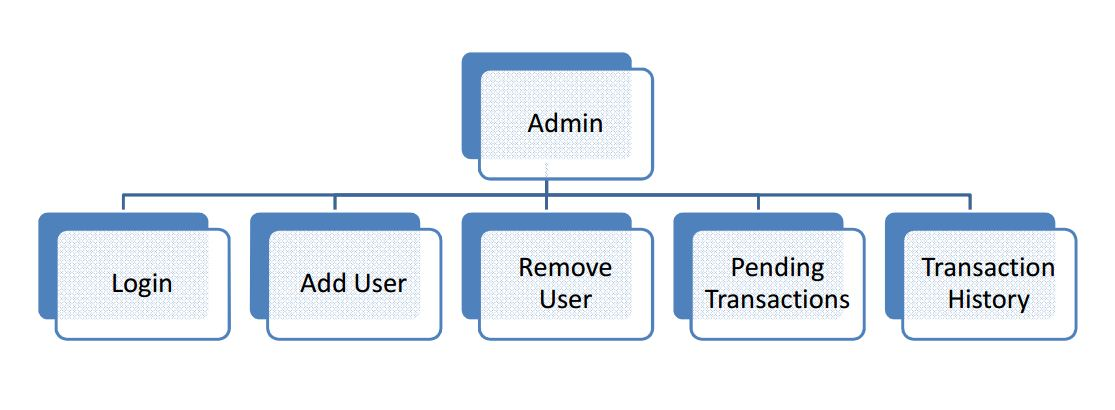
\includegraphics[width=6in]{block1.jpg} 
	\caption{Admin}
  \centering
    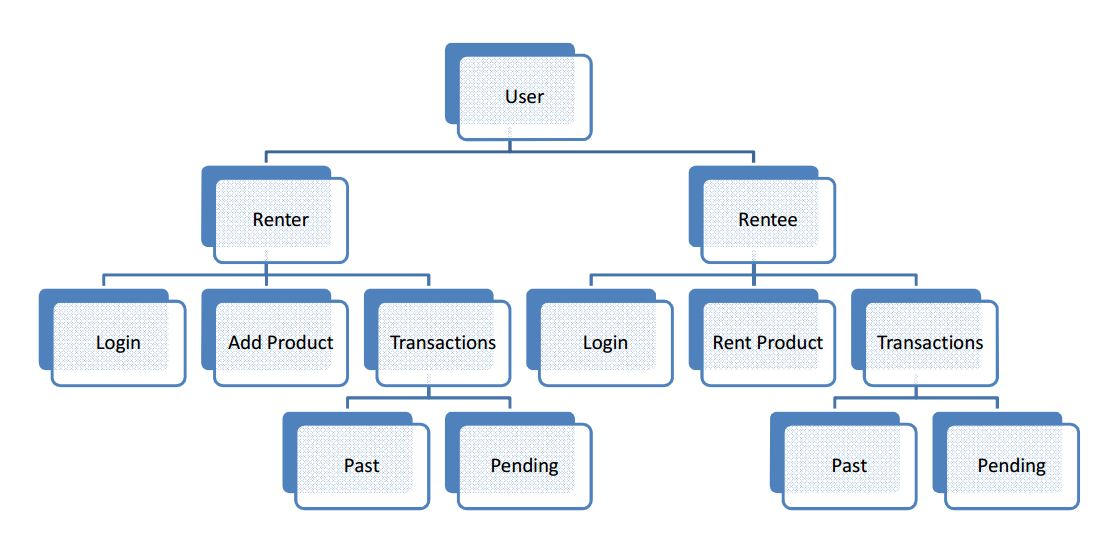
\includegraphics[width=6in]{block2.jpg} 
	\caption{User}
\end{figure}
%%%%%%%%%%%%
\begin{figure}[h]
\section{Dataflow Diagrams}
  \centering
    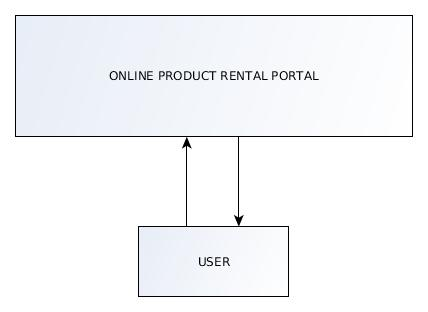
\includegraphics[width=3in]{level0.jpg} 
	\caption{Level 0 DFD}
% should be 1.1
\vspace{1cm}
  \centering
    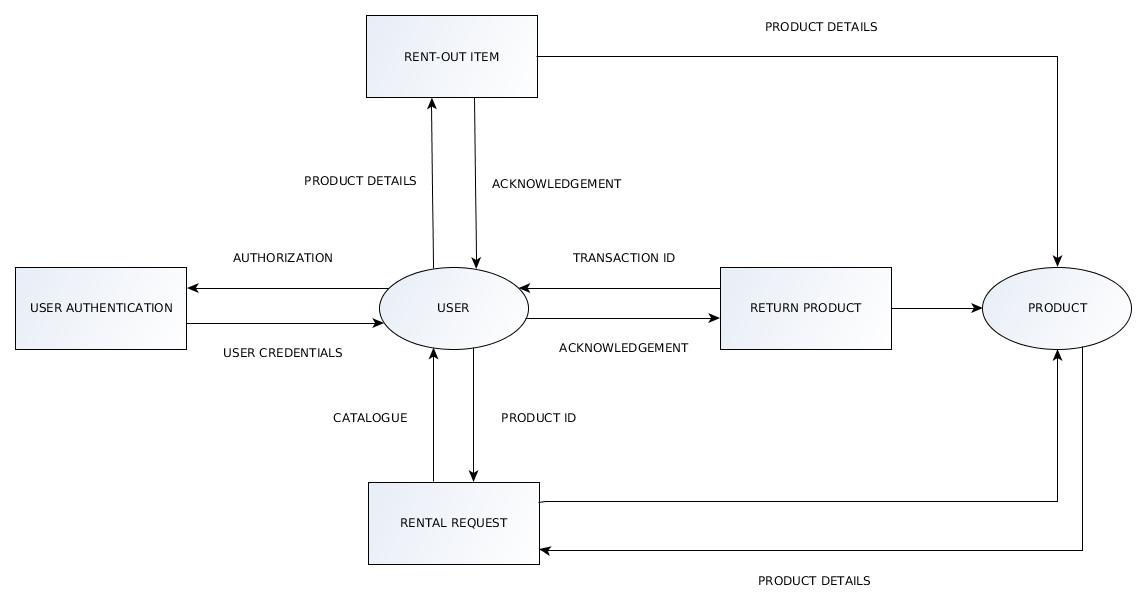
\includegraphics[width=\textwidth]{level1.jpg} 
	\caption{Level 1 DFD}
\end{figure}
% should be 1.1

%\epsfig{width=8in,height=6in, file=co.png}

%%%%%%%%%%%%%%%%


\begin{figure}[h]
\section{Algorithms}
%optional
We have mainly four types of algorithms, administrator tasks, renter specific algorithms, rentee specific algorithms and some that are applicable to all three categories.\\

\subsection{Administrator}
%optional
\subsubsection{Admin Login}
\begin{tabbing}
\= xxx\= \kill
function adminLogin (email, password)\\
\{\\
\hspace{0.3in}connect to DB\\
\hspace{0.3in}if (email exists in DB) \{\\
 \hspace{0.6in}if (password is correct)\\ 
\hspace{1.2in}return true ;\\
\hspace{0.3in} \}
\hspace{0.3in}return false;\\
\}
\end{tabbing}
\subsubsection{Close Complaint}
\begin{tabbing}
\= xxx\= \kill
function closeComplaint (productID, renteeID)\\
\{\\
\hspace{0.3in}connect to DB\\
\hspace{0.3in}if (complaint where renteeID and productID matches exists) \{\\
 \hspace{0.6in}if (loggedin)\{\\ 
\hspace{1.2in}Remove record from complaints;\\
\hspace{1.2in};Update transaction history\\
\hspace{1.2in}return true;\\
\hspace{0.6in} \}\\
\hspace{0.3in} \}\\
\hspace{0.3in}return false;\\
\}
\end{tabbing}
\end{figure}
\begin{figure}[h]
\subsection{Renter}
\subsubsection{Rent Out Product}
\begin{tabbing}
\= xxx\= \kill
function rentOut (product, renterID)\\
\{\\
\hspace{0.3in}connect to DB\\
\hspace{0.3in}if (renterID exists in DB) \{\\
 \hspace{0.6in}if (loggedin)\{\\ 
\hspace{1.2in}create new product entry in DB ;\\
\hspace{1.2in}return true;\\
\hspace{0.6in} \}\\
\hspace{0.3in} \}\\
\hspace{0.3in}return false;\\
\}
\end{tabbing}
\subsubsection{Add Complaint}
\begin{tabbing}
\= xxx\= \kill
function addComplaint (productID, renteeID,complaint)\\
\{\\
\hspace{0.3in}connect to DB\\
\hspace{0.3in}if (transaction where renteeID and productID matches exists) \{\\
 \hspace{0.6in}if (loggedin)\{\\ 
\hspace{1.2in}Add new entry in Complaints for the given product;\\
\hspace{1.2in}Update transaction history;\\
\hspace{1.2in}Remove record from Transactions;\\
\hspace{1.2in}return true;\\
\hspace{0.6in} \}\\
\hspace{0.3in} \}\\
\hspace{0.3in}return false;\\
\}
\end{tabbing}
\end{figure}
\begin{figure}[h]
\subsection{Rentee}
\subsubsection{Rent In Product}
\begin{tabbing}
\= xxx\= \kill
function rentIn (product, userID)\\
\{\\
\hspace{0.3in}connect to DB\\
\hspace{0.3in}if (product exists in DB) \{\\
 \hspace{0.6in}if (loggedin)\{\\ 
\hspace{1.2in}Update product status as not available;\\
\hspace{1.2in}Add transaction entry with status pending\\
\hspace{1.2in}Add history entry with current timestamp;\\
\hspace{1.2in}return true;\\
\hspace{0.6in} \}\\
\hspace{0.3in} \}\\
\hspace{0.3in}return false;\\
\}
\end{tabbing}
\subsubsection{Approve/Reject Product}
\begin{tabbing}
\= xxx\= \kill
function appReject (product, userID,apporrej)\\
\{\\
\hspace{0.3in}connect to DB\\
\hspace{0.3in}if (product exists in transaction DB) \{\\
 \hspace{0.6in}if (loggedin)\{\\ 
\hspace{1.2in}if (approved)\{\\ 
\hspace{1.5in} Update transaction status as rented;\\
\hspace{1.5in}Update history entry with current timestamp;\\
\hspace{1.2in} \}else\{\\
\hspace{1.5in}Remove transaction entry;\\
\hspace{1.2in} \}\\
\hspace{1.2in}return true;\\
\hspace{0.6in} \}\\
\hspace{0.3in} \}\\
\hspace{0.3in}return false;\\
\}
\end{tabbing}
\end{figure}
\begin{figure}[h]
\subsection{Miscellaneous}
\subsubsection{User Signup}
\begin{tabbing}
\= xxx\= \kill
function Signup (email, password,details)\\
\{\\
\hspace{0.3in}connect to DB\\
\hspace{0.3in}if (email does not exist in DB) \{\\
 \hspace{0.6in}Add new user entry;\\ 
 \hspace{0.6in}Add new user details;\\ 
 \hspace{0.6in}Hash and store password;\\ 
\hspace{0.6in}return true ;\\
\hspace{0.3in} \}\\
\hspace{0.3in}return false;\\
\}
\end{tabbing}
\subsubsection{User Login}
\begin{tabbing}
\= xxx\= \kill
function userLogin (email, password)\\
\{\\
\hspace{0.3in}connect to DB\\
\hspace{0.3in}if (email exists in DB) \{\\
 \hspace{0.6in}if (password is correct)\\ 
\hspace{1.2in}return true ;\\
\hspace{0.3in} \}
\hspace{0.3in}return false;\\
\}
\end{tabbing}
\subsubsection{User Logout}
\begin{tabbing}
\= xxx\= \kill
function userLogout ()\\
\{\\
\hspace{0.3in}connect to DB\\
\hspace{0.3in}Destroy current session;\\
\hspace{0.3in}return true;\\
\}
\end{tabbing}
\end{figure}
%%%%%%%%%%

\begin{figure}[h]
\section{Database Design}
Data is stored in the server machine with the aid of mySql database.\\
\subsection{Database Tables}
  \centering
    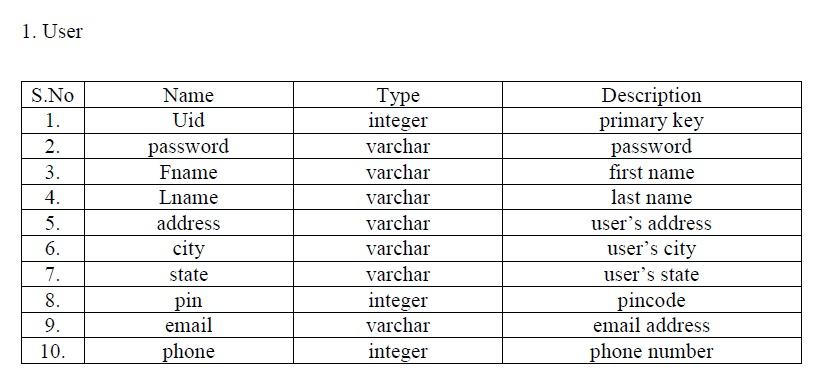
\includegraphics[width=7in]{user.jpg} 
  \centering
    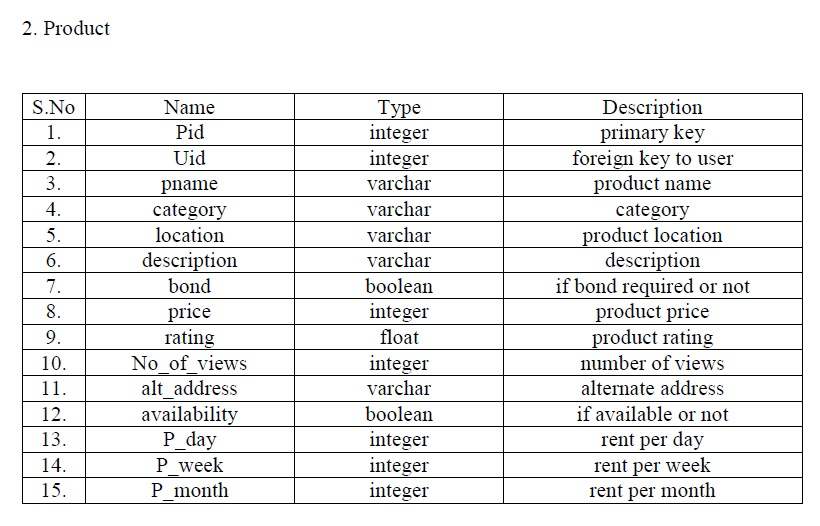
\includegraphics[width=7in]{product.jpg} 
   \end{figure}
\begin{figure}[h]
  \centering
    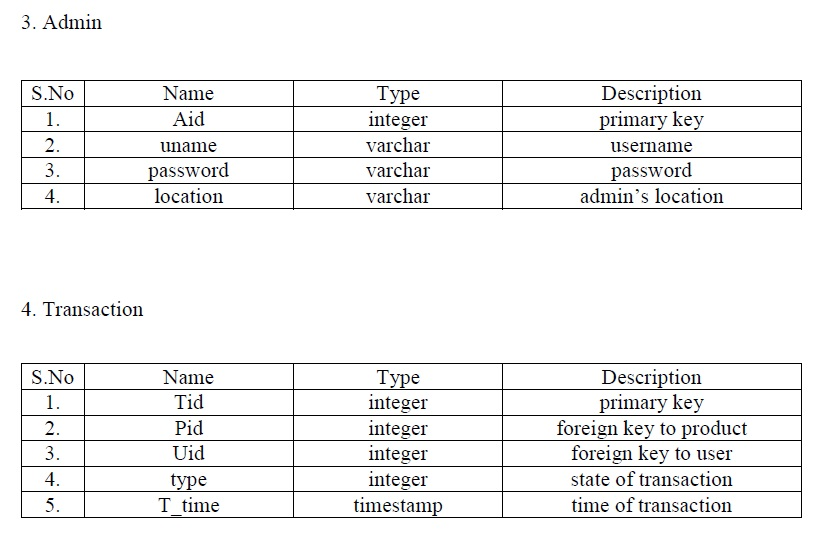
\includegraphics[width=7in]{admin_transaction.jpg} 
  \centering
    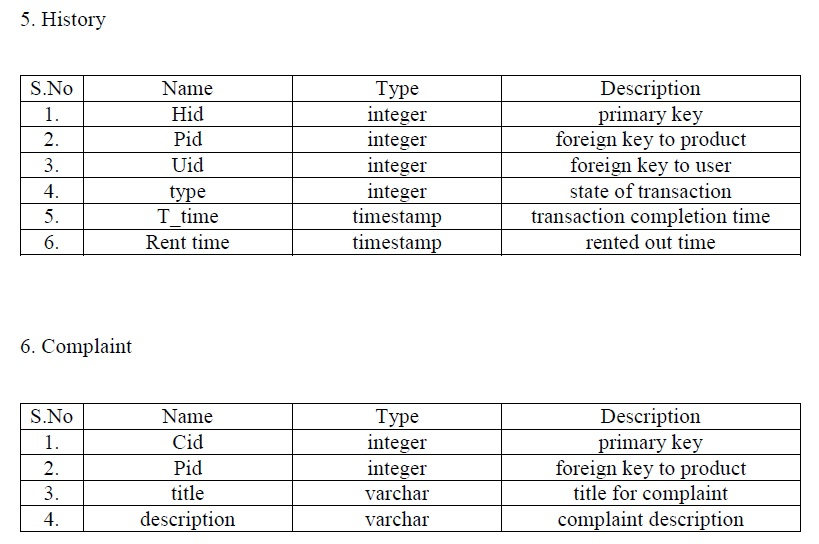
\includegraphics[width=7in]{history_complaint.jpg} 
   \end{figure}
\begin{figure}[h]
  \centering
    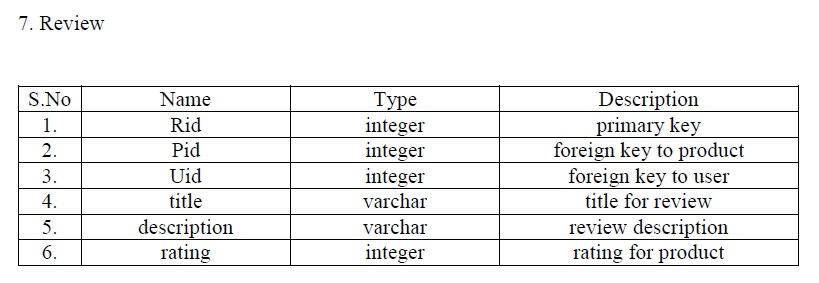
\includegraphics[width=7in]{review.jpg} 
    \vspace{10in}
   \end{figure}
\begin{figure}[h]   
\subsection{ER Diagram}
Various entities used in product are:
\begin{enumerate}
\item{Admin}
\item{User}
\item{Product}
\item{Transaction}
\item{History}
\item{Complaint}
\item{Review}
\end{enumerate}
  \centering
    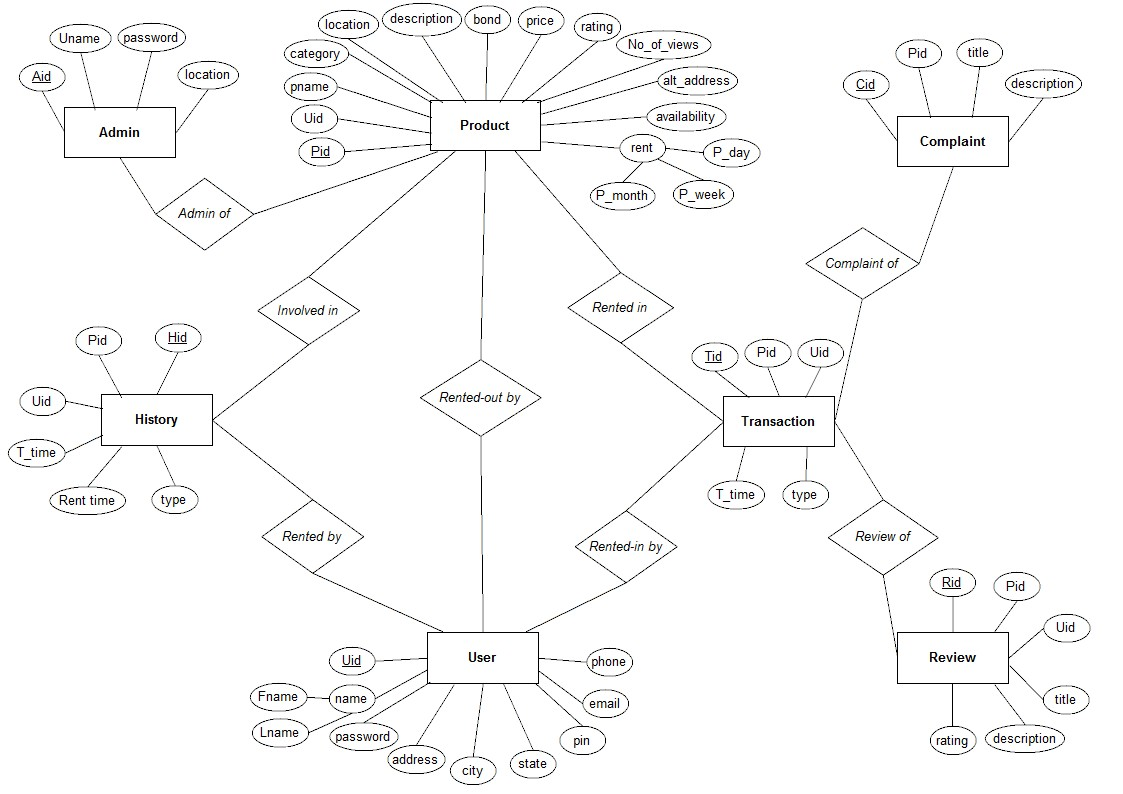
\includegraphics[width=7in]{erdgm.jpg} 
	\caption{ER Diagram}
\end{figure}
\begin{figure}[h]
\section{Human Interface Design}

\subsection{Overview of User Interface}
User logs in to the website using his/her email id and password. On logging in the user will be directed to the homepage where the product catalogue is displayed along with search and navigation options . Additionally he can navigate to check/update the status of his account. Also he can check his rental history. Furthermore, the user  can add products to be rented out. 
\\Administrators will login to a separate page where he can carry out administrative tasks such as editing user/product details , updating complaint status, etc.\\
All pages in the portal are mobile-friendly.\\
\subsection{Screen Images}
\vspace{0.5in}
  \centering
    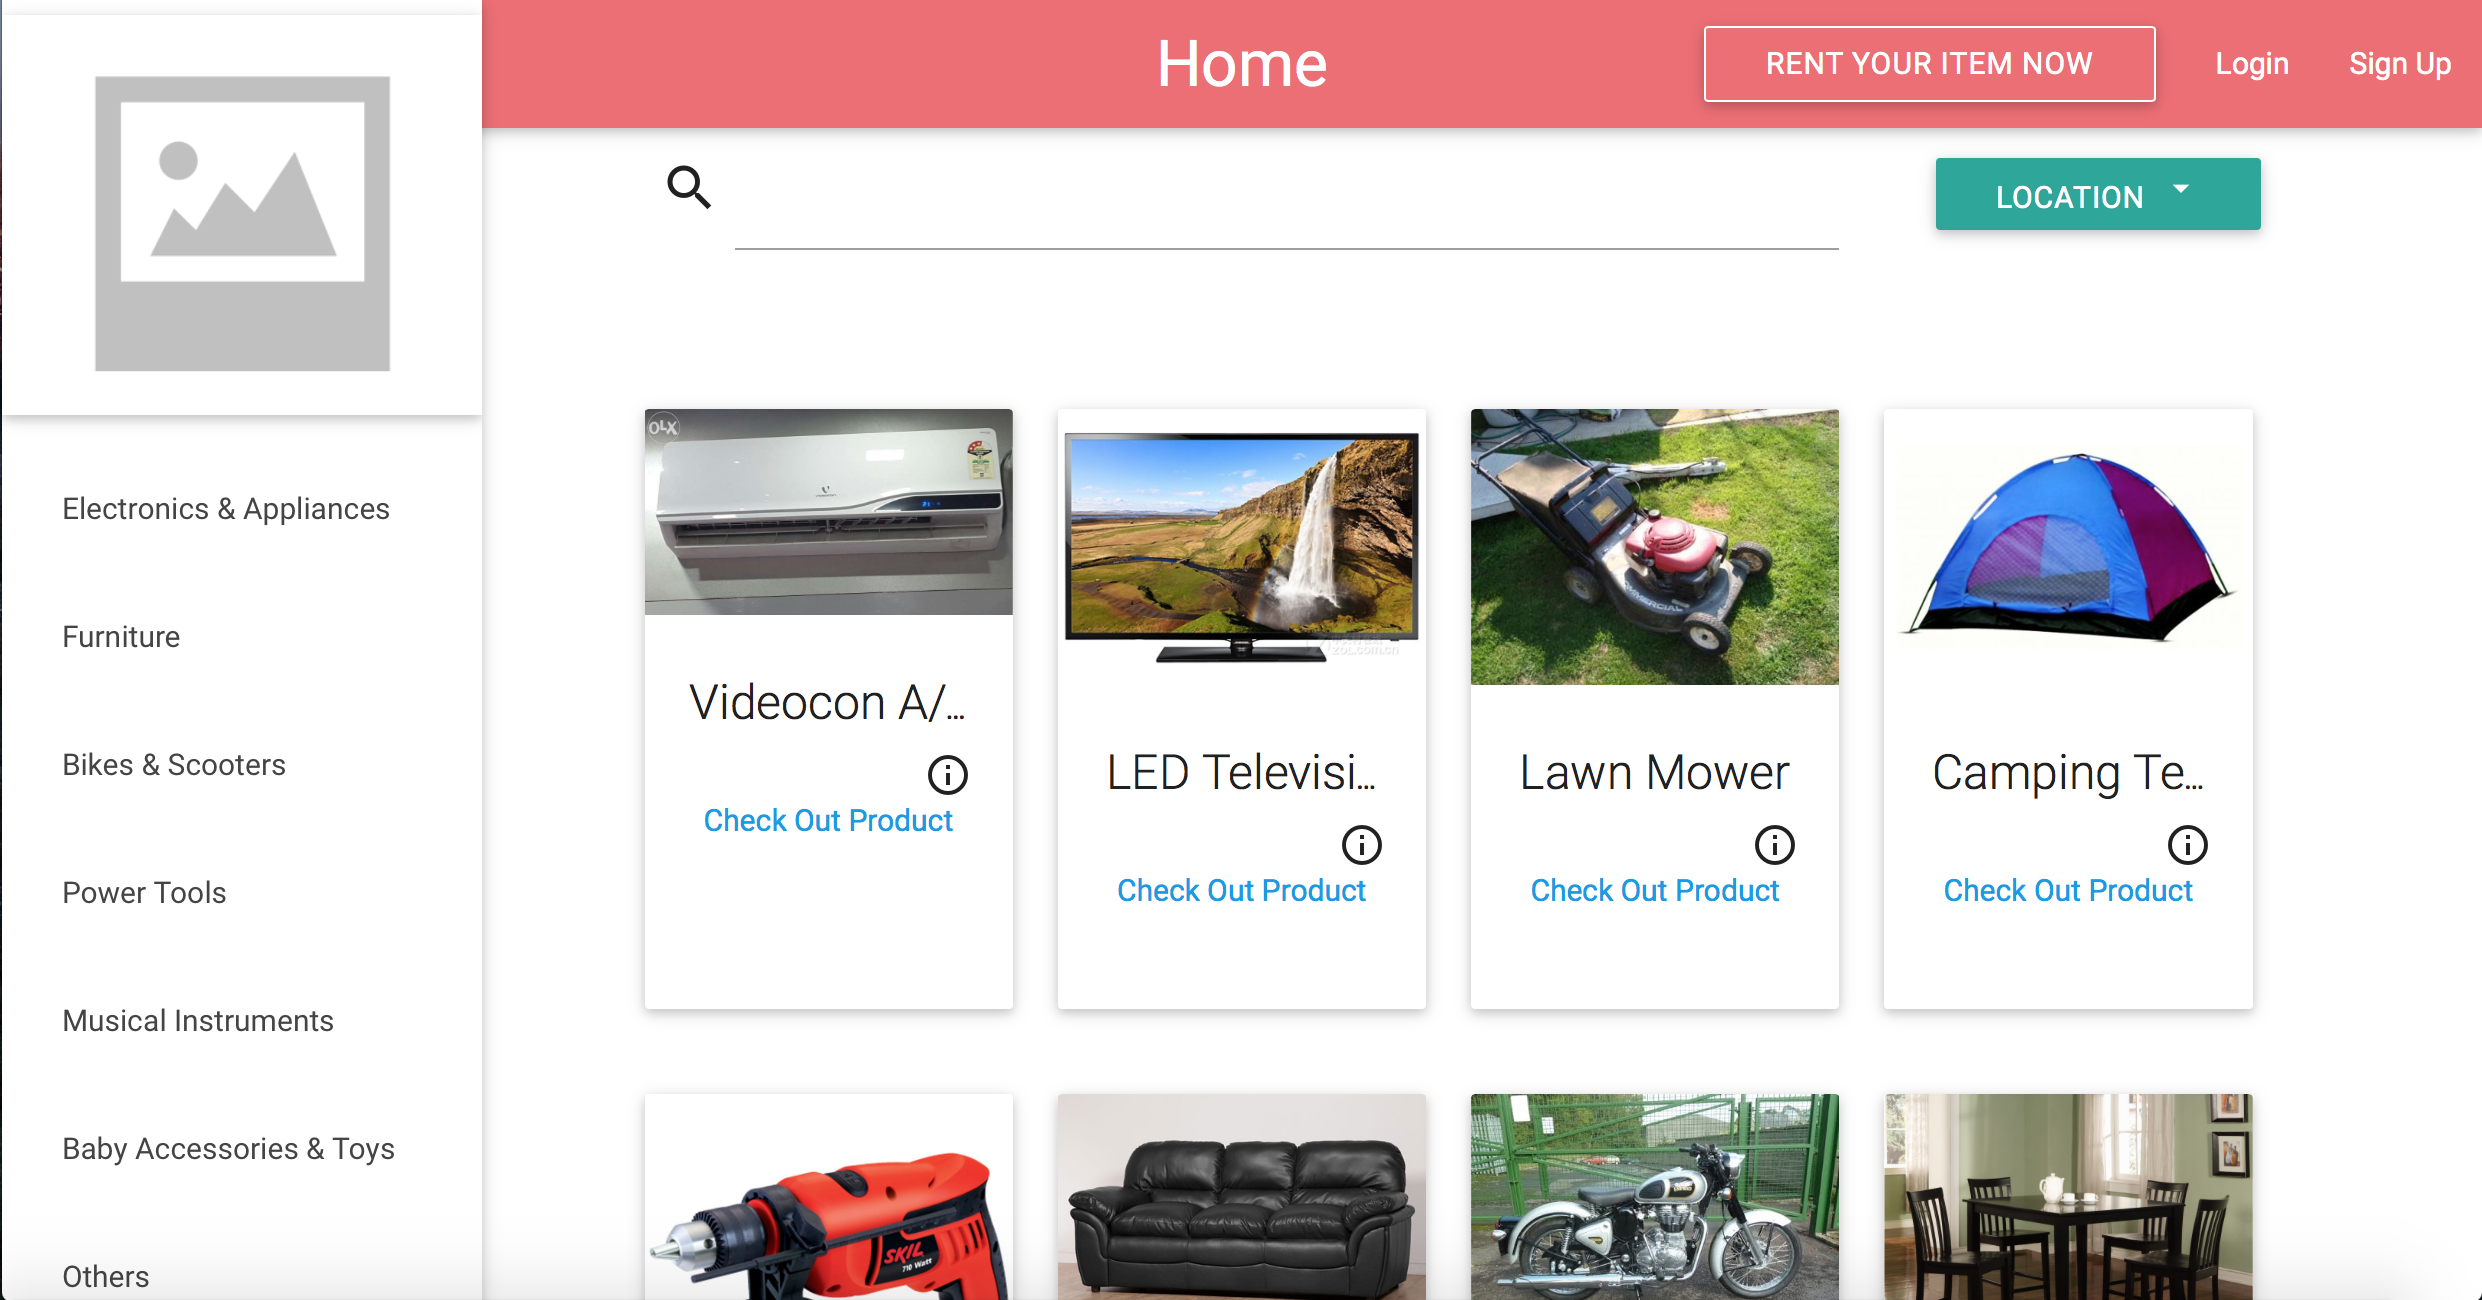
\includegraphics[width=6in]{homepage.png} 
    \end{figure}
    \begin{figure}[h]
  \centering
    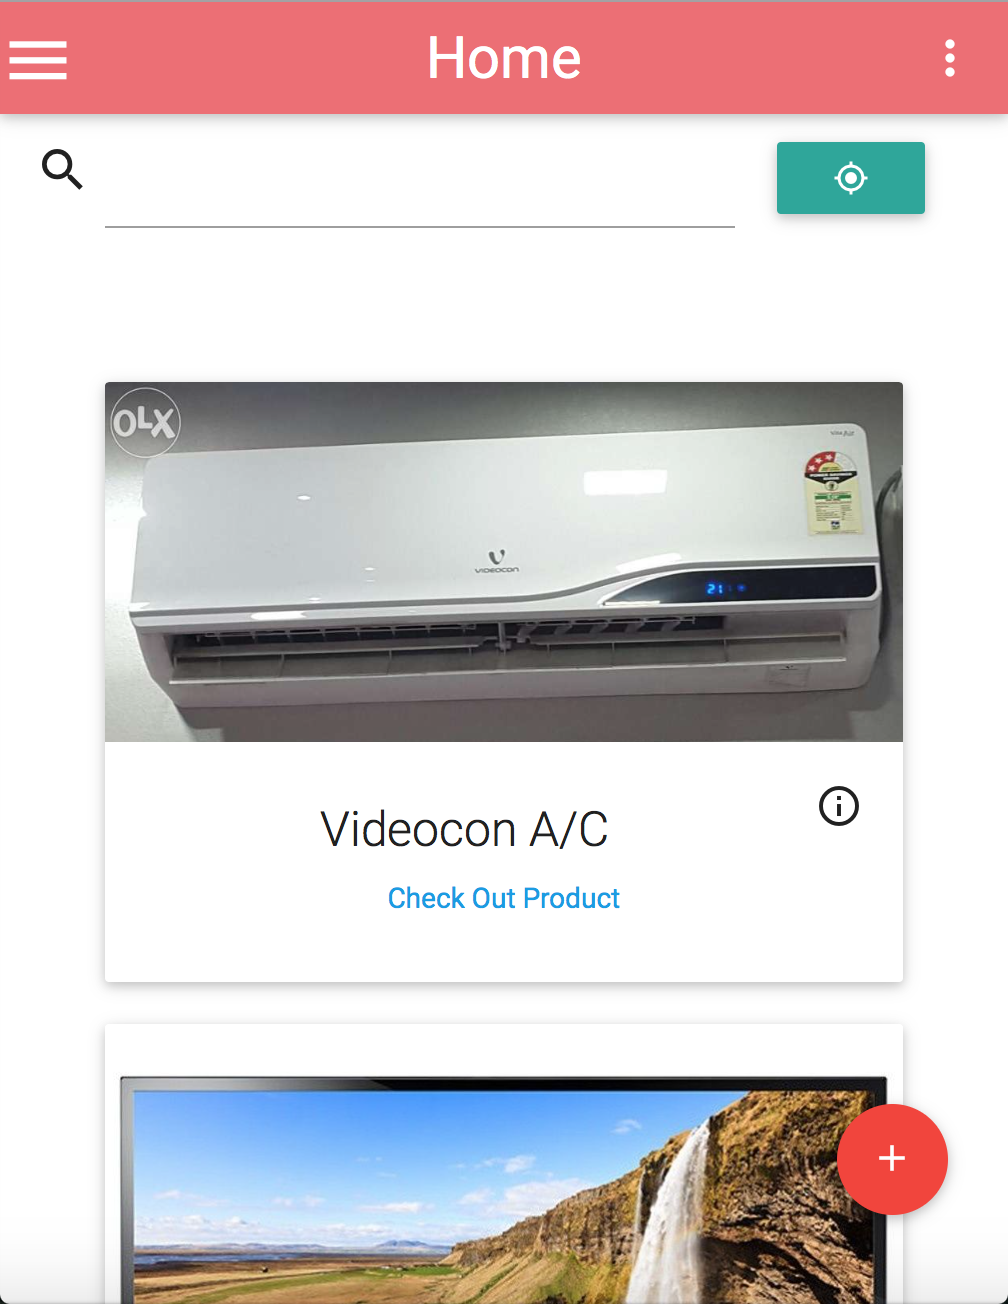
\includegraphics[width=4in]{homepage_mobile.png} 
	\caption{Homepage}
	\end{figure}
    \begin{figure}[h]
\vspace{0.5in}
  \centering
    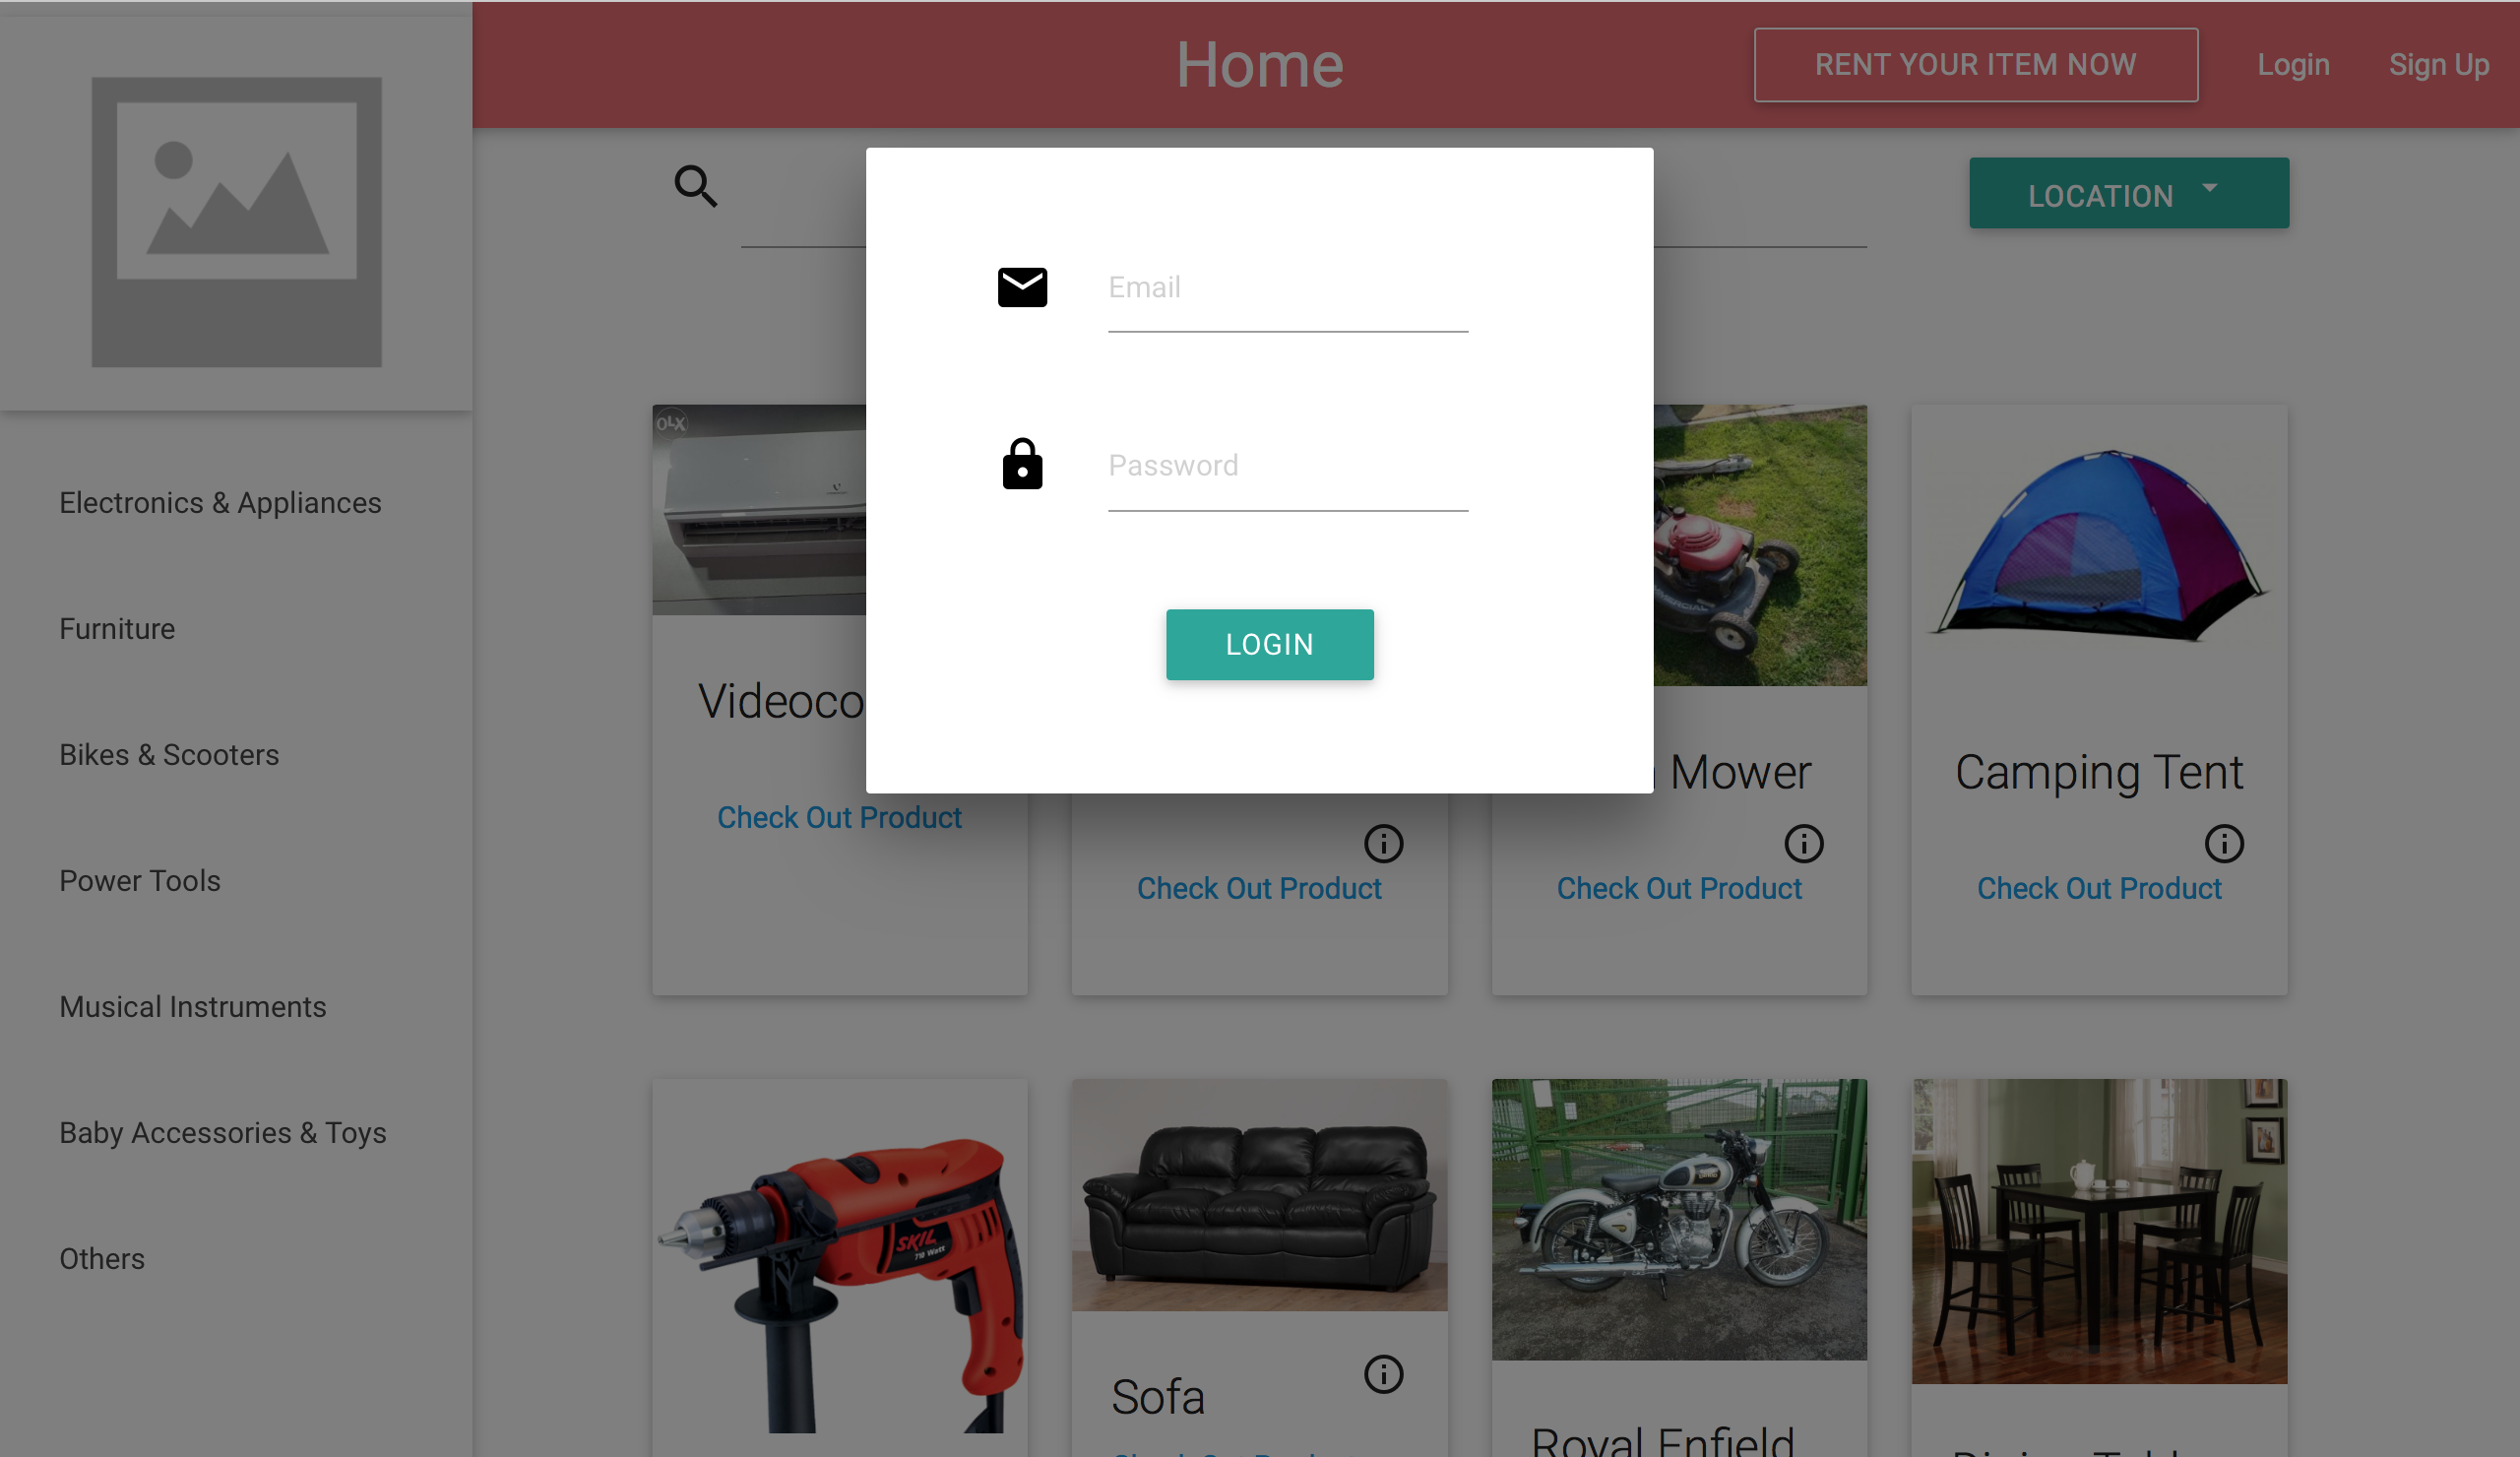
\includegraphics[width=4in]{login.png} 
	\caption{Login Screen}
	\end{figure}
\begin{figure}[h]
\subsection{Screen Objects and Actions}
\textbf{Home Screen}
\begin{enumerate}
\item{Login : Modal for login pops up}
\item{Signup : Modal for signup pops up}
\item{Search : Search for products based on location}
\item{Navigation : Navigate to different category  pages}
\item{Checkout Product : Navigate to the product's page}
\item{Rent Item Now : Add product to be rented out}
\end{enumerate}
\end{figure}
\begin{figure}[h]
\textbf{Login Screen}
\begin{enumerate}
\item{Email ID : Used to enter the user email id}
\item{Password : Used to enter password}
\item{Login Button : Log in to the portal}
\end{enumerate}
\end{figure}

%======================================================

\chapter{Implementation}
% detailed description on implementation

\section{Overview of Technologies Used}
% give the overview of different technologies/ frameworks/ packages used for your project in neat and clean manner with proper headings and subheadings. ( eg: .NET / Java / GTK etc)
\subsection{XAMP}
XAMP is a free and open source cross-platform web server solution stack package, consisting
mainly of the Apache HTTP Server, MySQL database, and interpreters for scripts written in the
PHP and Perl programming languages. X stands for Windows/Linux/Mac etc.

\subsection{MSMTP}
msmtp is an SMTP(Simple Mail Transfer Protocol) client.In the default mode, it transmits a mail to an SMTP server (for example at a free mail provider) which takes care of further delivery.\\Features include:
\begin{itemize}
  \item Sendmail compatible interface (command line options and exit codes)
  \item Support for multiple accounts
  \item TLS/SSL support including client certificates
  \item Many authentication methods
  \item Support for Internationalized Domain Names (IDN)
  \item Fast SMTP implementation using command pipelining
  \item DSN (Delivery Status Notification) support
  \item SOCKS proxy support
\end{itemize}
msmtp is free software; you can redistribute it and/or modify it under the terms of the GNU General Public License as published by the Free Software Foundation; either version 3 of the License, or (at your option) any later version.
\subsection{PHP}
PHP is a server-side scripting language designed for web development but also used as a general-
purpose programming language.PHP code can be simply mixed with HTML code, or it can be
used in combination with various templating engines and web frameworks. After the PHP code is
interpreted and executed, the web server sends resulting output to its client, usually in form of a
part of the generated web page.
\subsection{MySQL}
MySQL is the world’s second most widely used relational database management system (RDBMS)
and most widely used open-source RDBMS.MySQL is a popular choice of database for use in web
applications, and is a central component of the widely used XAMMP open source web application
software stack.
\subsection{Git}
Git is a widely used source code management system for software development. It is a distributed revision control system with an emphasis on speed,[6] data integrity, and support for distributed, non-linear workflows. Git was initially designed and developed in 2005 by Linux kernel developers for Linux kernel development. As Git is a distributed version control system, it can be used as a server out of the box. Dedicated Git server software helps, amongst other features, to add access control, display the contents of a Git repository via the web, and help managing multiple repositories. Bitbucket was the git client used for this project.
\subsection{Web Frontend Technologies}
\subsubsection{HTML}
HyperText Markup Language, commonly referred to as HTML, is the standard markup language used to create web pages. Along with CSS, and JavaScript, HTML is a cornerstone technology used to create web pages, as well as to create user interfaces for mobile and web applications. Web browsers can read HTML files and render them into visible or audible web pages. HTML describes the structure of a website semantically along with cues for presentation, making it a markup language, rather than a programming language.
%%%%%%

\subsubsection{CSS}
Cascading Style Sheets (CSS) is a style sheet language used for describing the presentation of a document written in a markup language. CSS is designed primarily to enable the separation of document content from document presentation, including aspects such as the layout, colors, and fonts. This separation can improve content accessibility, provide more flexibility and control in the specification of presentation characteristics, enable multiple HTML pages to share formatting by specifying the relevant CSS in a separate .css file, and reduce complexity and repetition in the structural content.

\subsubsection{JavaScript}
JavaScript is a high-level, dynamic, untyped, and interpreted programming language. It has been standardized in the ECMAScript language specification. Alongside HTML and CSS, it is one of the three essential technologies of World Wide Web content production; the majority of websites employ it and it is supported by all modern Web browsers without plug-ins. JavaScript is prototype-based with first-class functions, making it a multi-paradigm language, supporting object-oriented, imperative, and functional programming styles. It has an API for working with text, arrays, dates and regular expressions, but does not include any I/O, such as networking, storage, or graphics facilities, relying for these upon the host environment in which it is embedded.

\subsubsection{jQuery}
jQuery is a cross-platform JavaScript library designed to simplify the client-side scripting of HTML.[2] jQuery is the most popular JavaScript library in use today.  jQuery is free, open-source software licensed under the MIT License.

\subsubsection{Materializecss}
Created and designed by Google, Material Design is a design language that combines the classic principles of successful design along with innovation and technology. Google's goal is to develop a system of design that allows for a unified user experience across all their products on any platform. Materializecss is a modern responsive front-end framework based on Material Design.
\section{Testing}
% give the overview about the tests you performed for your project  and your test plan

\subsection{Types of Testing}
\subsubsection{Alpha Testing}
We populated the database with different users and products (along with other resources such as images etc.) and then tried carried out the different operations such as renting items out and renting them in. The working of automatic mail was checked and the entire flow of transaction was also verified.
%%%%%
\subsubsection{Beta Testing}
The product was distributed among a selected group of individuals and tested for any possible
bugs. Administration using the admin dashboard was also done in this phase.
\section{Results}
% screenshots of your system with proper subtitles.


%==========================================================
\chapter{Conclusion}
\label {con}
\section{Conclusion}
With this product rental portal implemented, a lot of unused products can be turned into a form of passive revenue. Also the costs of buying, shipping and packaging a new product can be reduced.
% conclusion
\section{Future Scope}
% future enhancements possible    
This product can be upgraded in the future to include a feature to provide various other services like plumbers, electricians, gardeners etc. for daily wages managed by the web app.
%============================================================

\begin{thebibliography}{}

\addcontentsline{toc}{chapter}{References}

\bibitem{1} \textquotedblleft XAMPP Installers and Downloads for Apache Friends \textquotedblright[Online].\\ 
Available: $https://www.apachefriends.org/$

\bibitem{2} \textquotedblleft PHP: Hypertext Preprocessor \textquotedblright[Online].\\ 
Available: $http://www.php.net/$

\bibitem{3} \textquotedblleft Materialize design in css \textquotedblright [Online].\\
Available: $http://materializecss.com/$

\bibitem{4} \textquotedblleft Msmtp: An SMTP Client \textquotedblright [Online].\\
Available: $http://msmtp.sourceforge.net/$

\end{thebibliography}


\end{document}
